%%%%%%%%%%%%%%%%%%%%%%%%%%%%%%%%
\section{The 35-t Prototype}
\label{sec:proto-35t}

The 35-t (metric ton) LAr prototype was initially conceived to demonstrate that a non-evacuable
membrane cryostat could satisfy the DUNE far detector requirement that oxygen contamination
of the LAr be less than 200 parts per trillion (ppt), and that such a cryostat
could stably maintain that level.  In addition, construction and operation of the
35-t cryostat also served to identify requirements for procurement of materials and services,
to inform procedures for construction, and to inform best practices for safe operation.
Construction and operation of the 35-t membrane cryostat alone, now called ``Phase-1,''
was successfully completed in 2014.

The scope of the 35-t prototype was extended to a second phase, with the decision to install
and operate a small-scale, single-phase LArTPC and photon detector in the membrane cryostat.
Phase 2 focuses on the performance of active detector elements within the LAr volume.
Phase-2 is currently under construction and plans to take data in summer 2015.

\subsection{35-t Phase-1}

The 35-t membrane cryostat was built by a Japanese company, IHI\cite{bib:ihicorp},
contracted by the LBNE project.  
Table~\ref{tab:35Tdimensions} lists the construction materials and the
dimensions for the 35-t prototype; more information can be found in~\cite{bib:membcryo1573}.
The prototype was built in Fermilab's PC-4 facility where the Liquid Argon Purity
Demonstrator (LAPD)~\cite{bib:lapdP07005} is also located, which allowed for re-use of a large portion
 of the cryogenic-process equipment installed for LAPD.  The proximity and size (30 tons) of the LAPD
 vessel also offered the possibility using LAPD as a partial storage vessel for LAr if it ever
 became necessary to empty the 35-t cryostat.

The 35-t system employed a submersible pump to move LAr from the cryostat to the filters.
Figure~\ref{fig:35cutaway} shows a cutaway view of the cryostat and a photograph of the interior
of the completed cryostat.

\begin{cdrfigure}[Cutaway view]{35cutaway}{(left) Cutaway view of the 35-t cryostat. (right) Interior
photograph of the completed cryostat.}
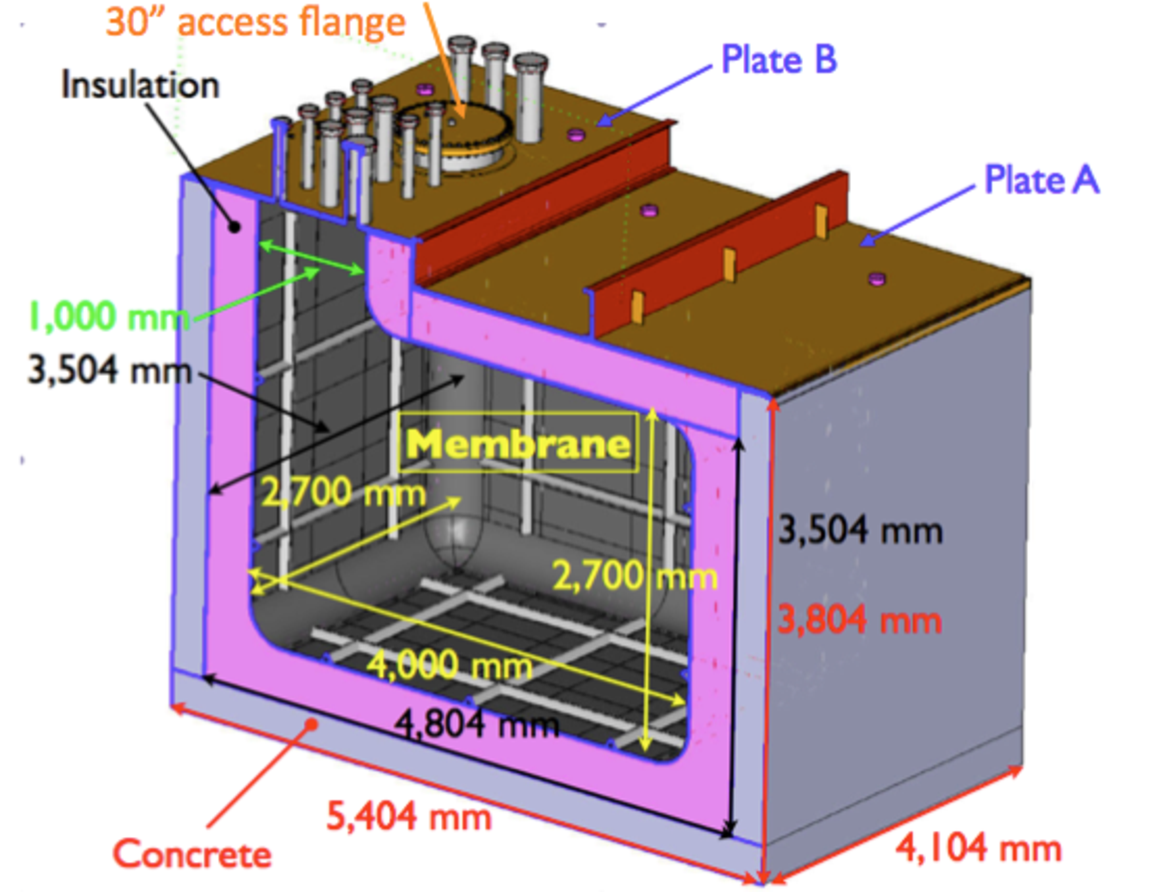
\includegraphics[width=0.60\textwidth]{35TCutaway}
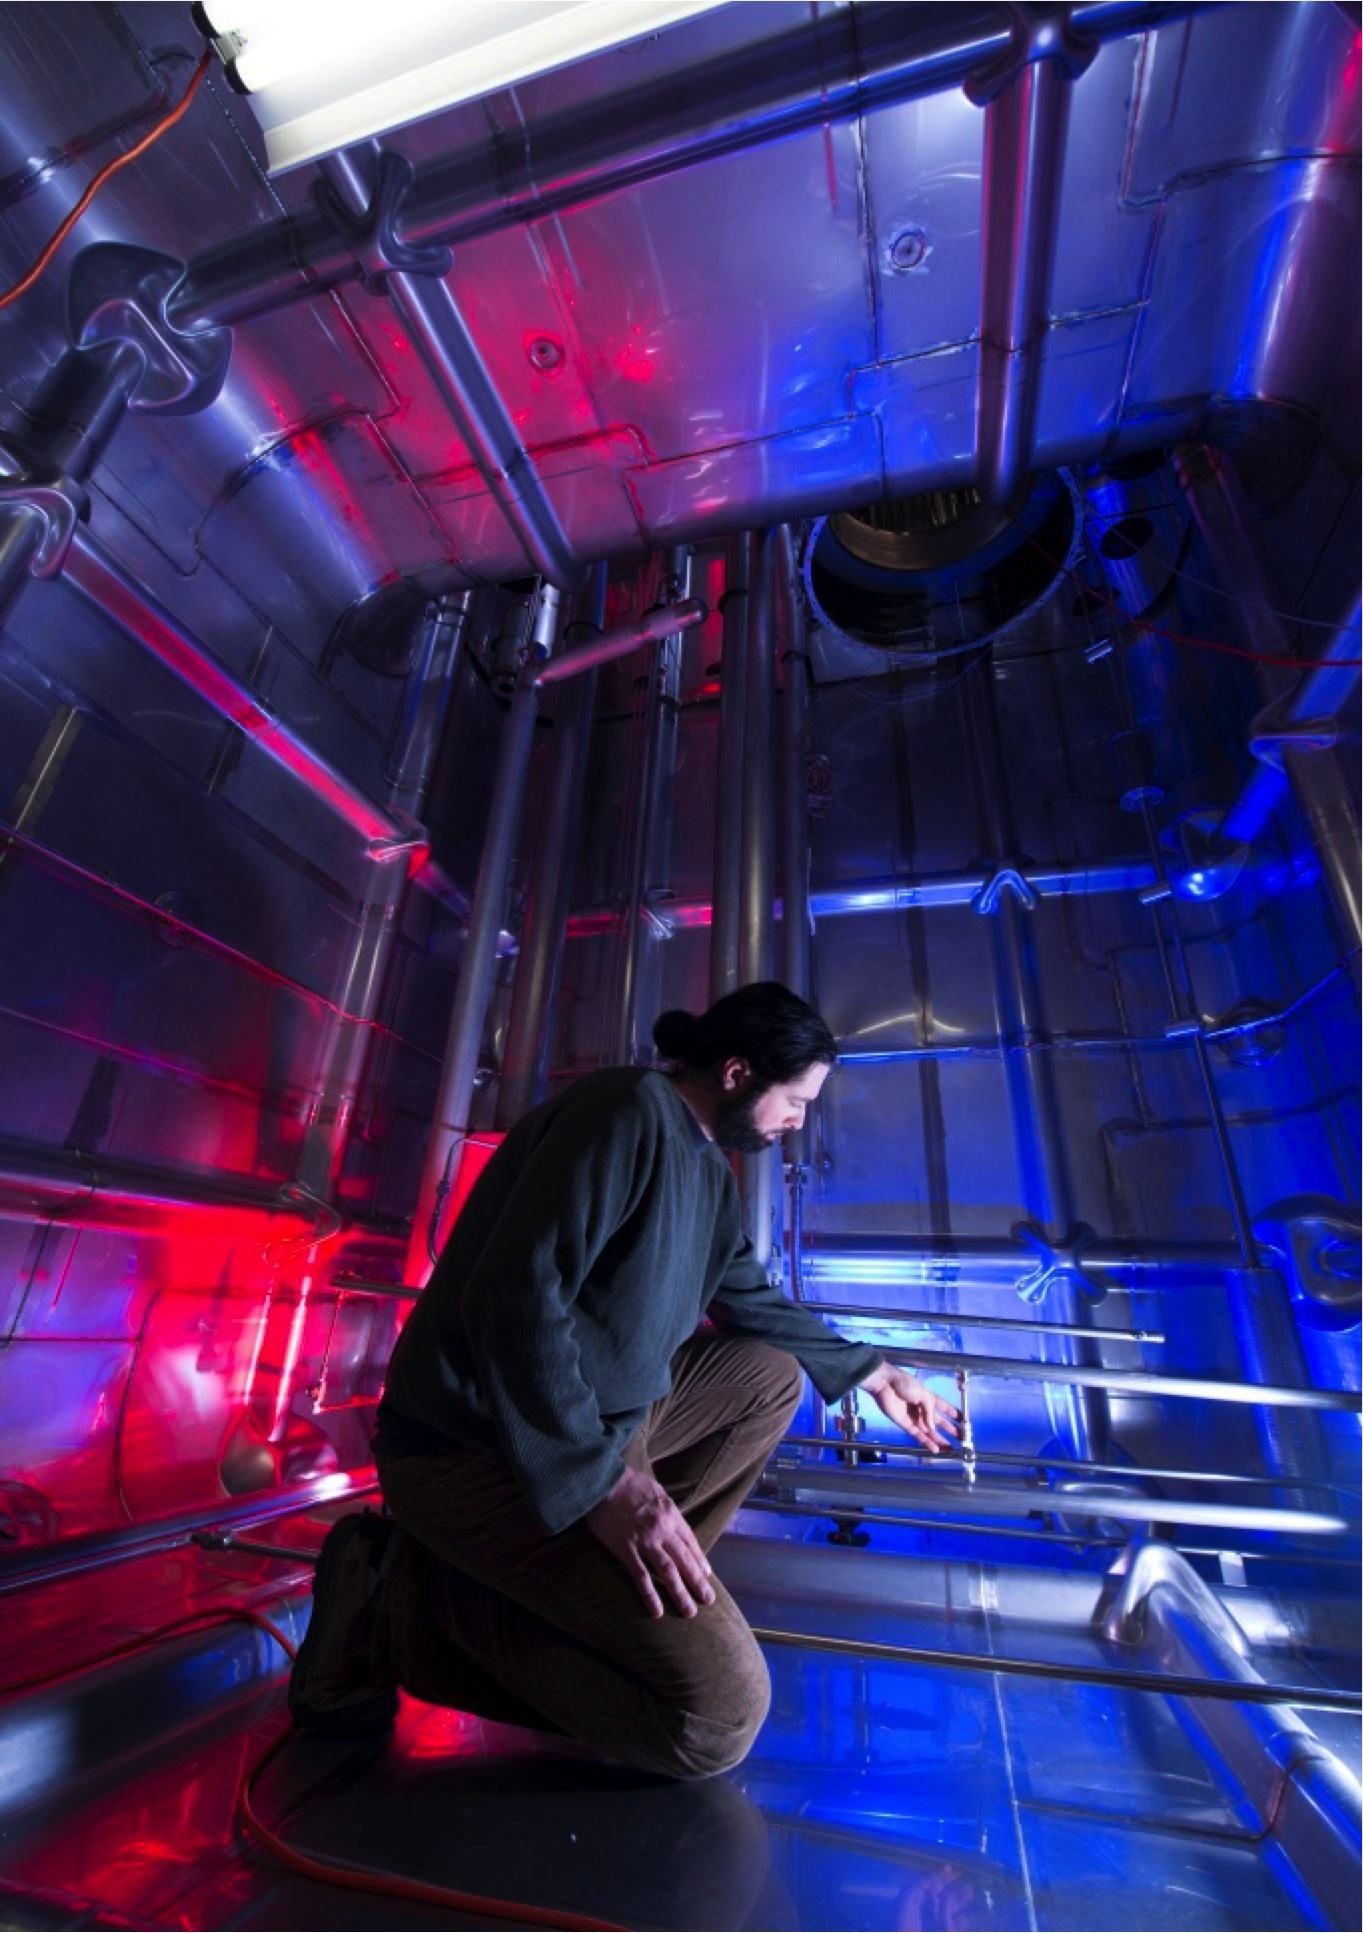
\includegraphics[width=0.35\textwidth]{35TCryo}
\end{cdrfigure}

The techniques of membrane cryostat construction were demonstrated to be suitable
for high-purity LArTPC service.  In particular, welding of corrugated panels, removal of leak-checking dye
penetrant and ammonia-activated leak-detecting paints, and post-construction-cleaning methods, were tested
and found to be suitable.

\begin{cdrtable}[35-t Prototype Materials and Dimensions]{ll}{35Tdimensions}
{35-t Prototype Materials and Dimensions}
Parameter & Value \\ \toprowrule
Cryostat Volume	&      29.16 m3\\ \colhline
Liquid argon total mass	 &     38.6 metric tons\\ \colhline
Inner dimensions	&      4.0 m (L) x 2.7 m (W) x 2.7 m (H)\\ \colhline
Outer dimensions        &      5.4 m (L) x 4.1 m (W) x 4.1 m (H)\\ \colhline
Membrane		&      2.0 mm thick corrugated 304 SS\\ \colhline
Insulation		&      0.4 m polyurethane foam\\ \colhline
Secondary barrier system	   &   0.1 mm thick fiberglass\\ \colhline
Vapor barrier	Normal	  &    1.2 mm thick carbon steel\\ \colhline
Steel reinforced concrete	    &  0.3 m thick layer\\
\end{cdrtable}

As was demonstrated by LAPD, initial removal of impurities within the cryostat can be
achieved by purging with gaseous argon. Accordingly, this 
was adopted for the 35-t as well.   Figure~\ref{fig:35TPurge} graphically shows the
first step of the purification process, removal of the ambient air.
The initial state, $t=0$, reflects the initial values for oxygen, water and
nitrogen in the ``dry air'' state.


\begin{cdrfigure}[Gas Ar Purge and Recirculation]{35TPurge}{Progress of the gas argon purge as it removes impurities  from the 35-t. The shown quantities are measured by various gas analyzers. The first stage of the purification is a process called the ``Piston Purge''.  The second stage is ``Recirculation with Filtering.'' The gap between the two steps was due to troubleshooting a leak.}
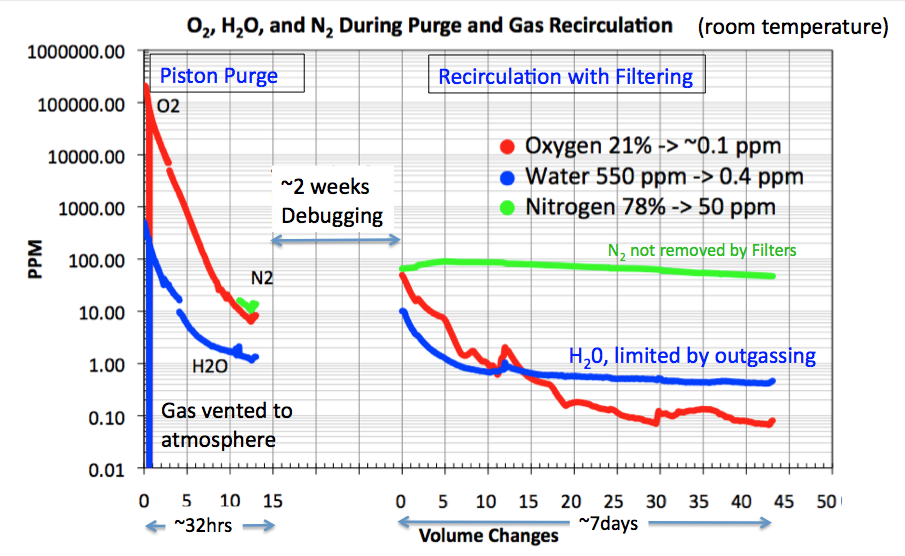
\includegraphics[width=0.8\textwidth]{35TPurgeAndRecirc}
\end{cdrfigure}

Once the room-temperature, gas purge was no longer improving purity,
the cooldown and LAr-fill stage began.
A gas/liquid spray method was used to cool the cryostat.
This generated a turbulent mixing of cold gas in the cryostat and cooled the entire surface.
The cooldown rate was maintained within the limits %below the maximum 
specified by the cryostat manufacturer.
Upon completion of the cooldown, LAr was transferred into the cryostat and %recirculating
purification via recirculation was begun. \fixme{check edit}

During recirculation and purification, dedicated purity monitors were used to measure electron lifetime, which can
be translated into equivalent oxygen contamination levels.
Figure~\ref{fig:35TElectronLifetime} shows the electron lifetime from the start of the
LAr pump operation until the end of the Phase-1 run.
In general, the electron lifetime improved as a function of pump
on-time; despite %there were also 
several events that spoiled the lifetime, %but 
the DUNE electron lifetime
specification (>1.4 ms) was easily achieved.

\begin{cdrfigure}[35t Electron Lifetime]{35TElectronLifetime}{LAr electron lifetmes as measured by
Cryostat Purity Monitors. Significant events are annotated on the plot. Major divisions on horizontal axis
are one week periods. Equivalent purity levels are shown as dashed horizontal lines.}
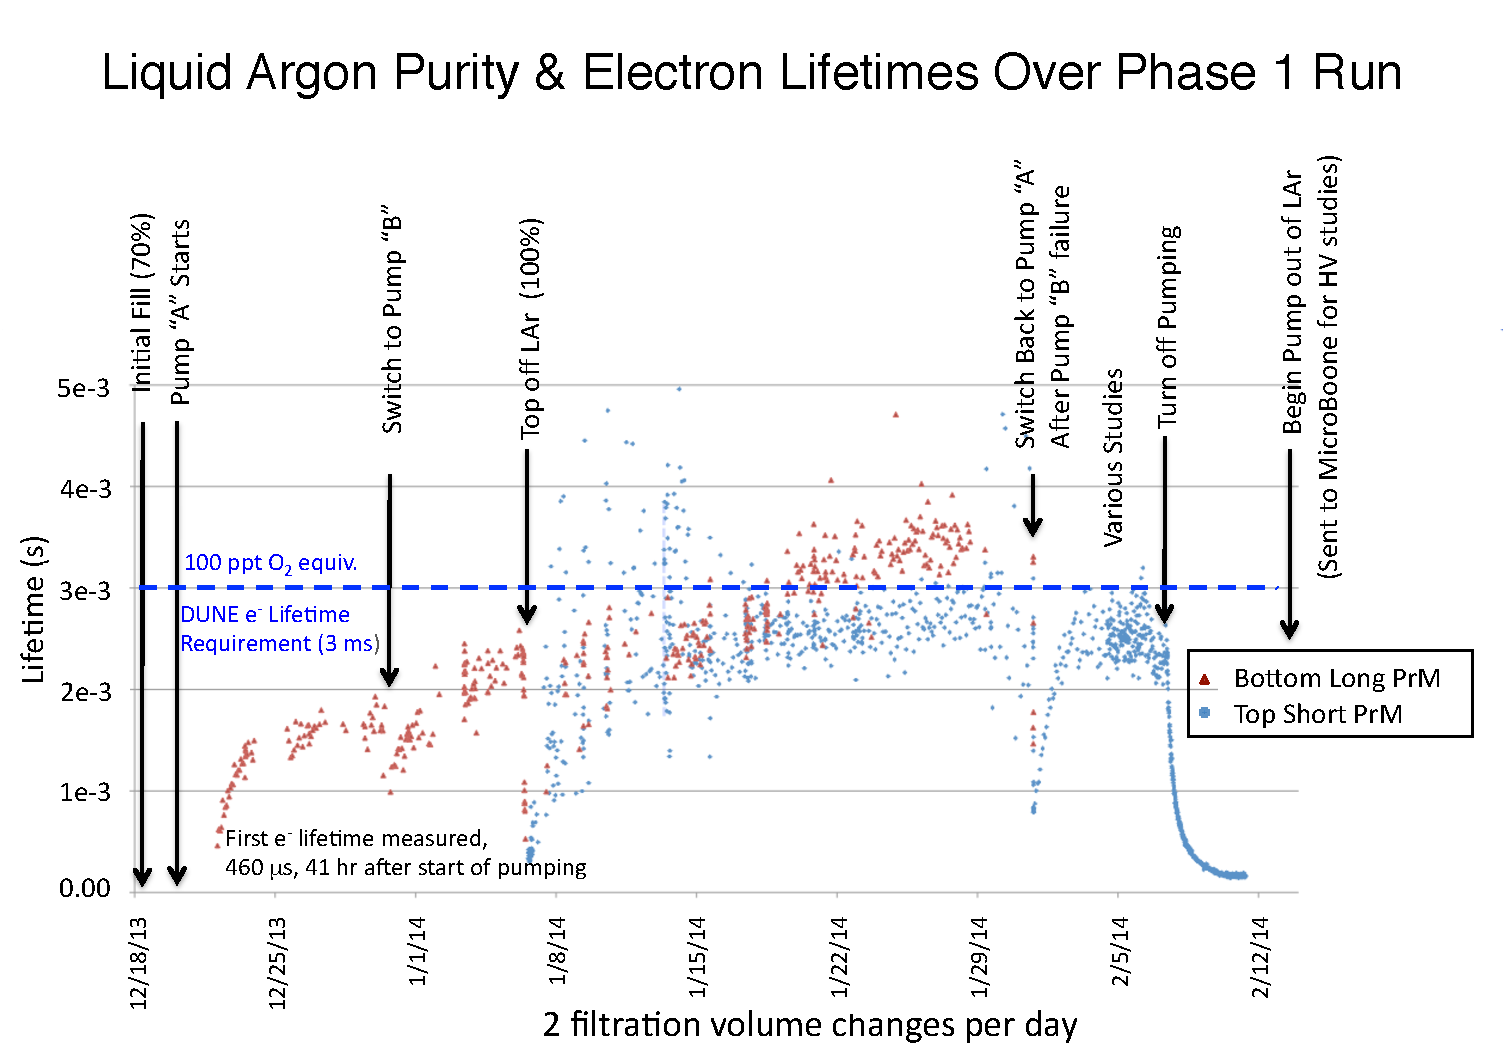
\includegraphics[width=0.7\textwidth]{35TElectronLifetime.pdf}
\end{cdrfigure}

The 35-t Phase-1 run successfully demonstrated that there is nothing %innate 
inherent to
membrane cryostat technology that would preclude achieving the stated goals of the
DUNE far detector. In addition, experience gained in operating the 35-t system
will inform future design decisions, e.g., finding an alternative to switching pumps, which
causes loss of purity. \fixme{check edit} %when switching pumps is
%undesirable, and can likely be avoided by improved system design. 
Future system
designs could also avoid the coupling of acoustical vibrations into the cryostat by %choosing to 
locating the pumps externally; this would have the added benefit of facilitating
maintenance and repair. 

\subsection{35-t Phase-2}
Phase-2 of the 35-t prototype cryostat extends its program %the scope   
to install %include 
a fully operational TPC and
photon detector in the %previously built Phase-1 
cryostat.
Installation of the TPC is expected in mid-2015 with commissioning to follow
after purge, cooldown and LAr fill.  Phase-2 operation is planned as a several-month-long
cosmic ray run.  External plastic scintillator paddles placed around the cryostat will provide
both the trigger for and rough position measurements of the incoming cosmic rays.

Figure~\ref{fig:tpc-35ton-trial} shows the trial assembly of the TPC outside of the cryostat.
Figure~\ref{fig:35TTPC} shows a model of the TPC inside the cryostat and a trial assembly of
the TPC done outside of the cyrostat.

\begin{cdrfigure}[35-t with TPC]{35TTPC}{(left) Rendering of the
35-t cryostat with TPC and photon detectors installed. 
Note the position of the APA, which is asymmetrically located and
splits the volume into two separate drift regions.
The length of the longer one of these is close to what is proposed for the far detector.
The other has a shorter drift length due to lack of space.
(right) A trial assembly of the TPC.
}
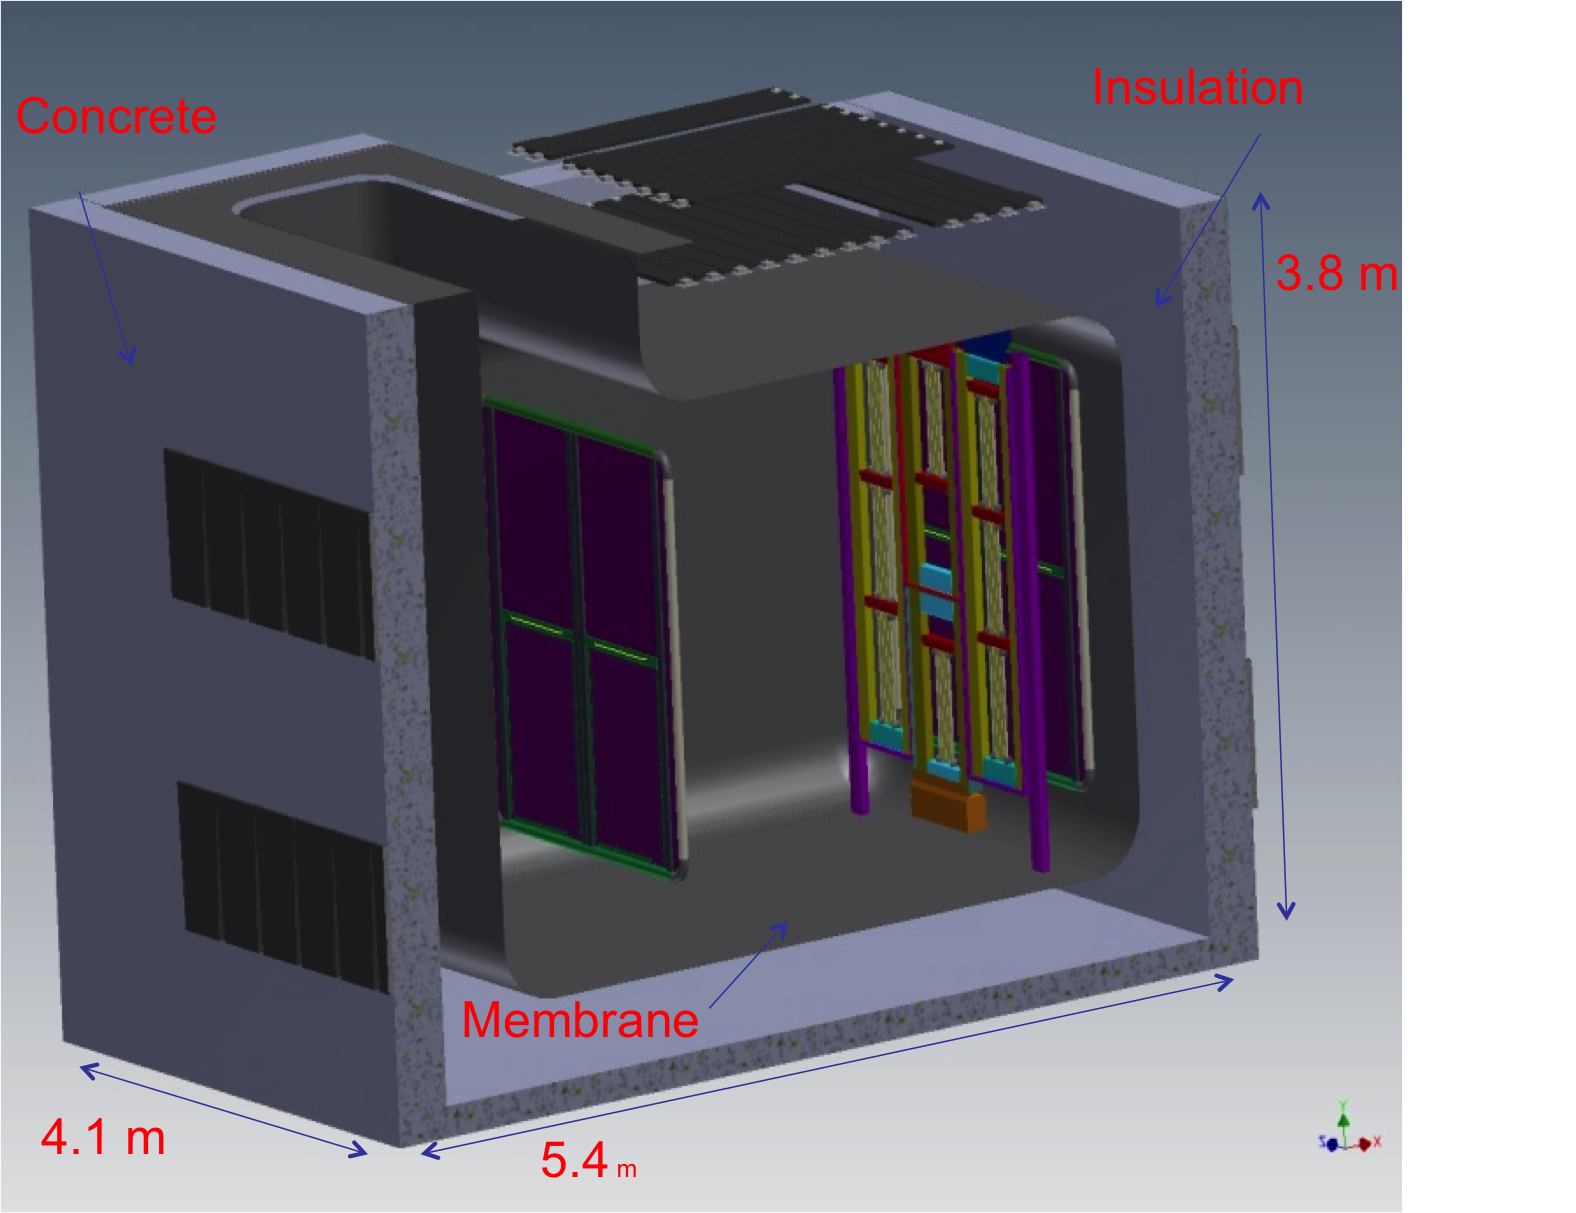
\includegraphics[width=0.55\textwidth]{35TTPC}
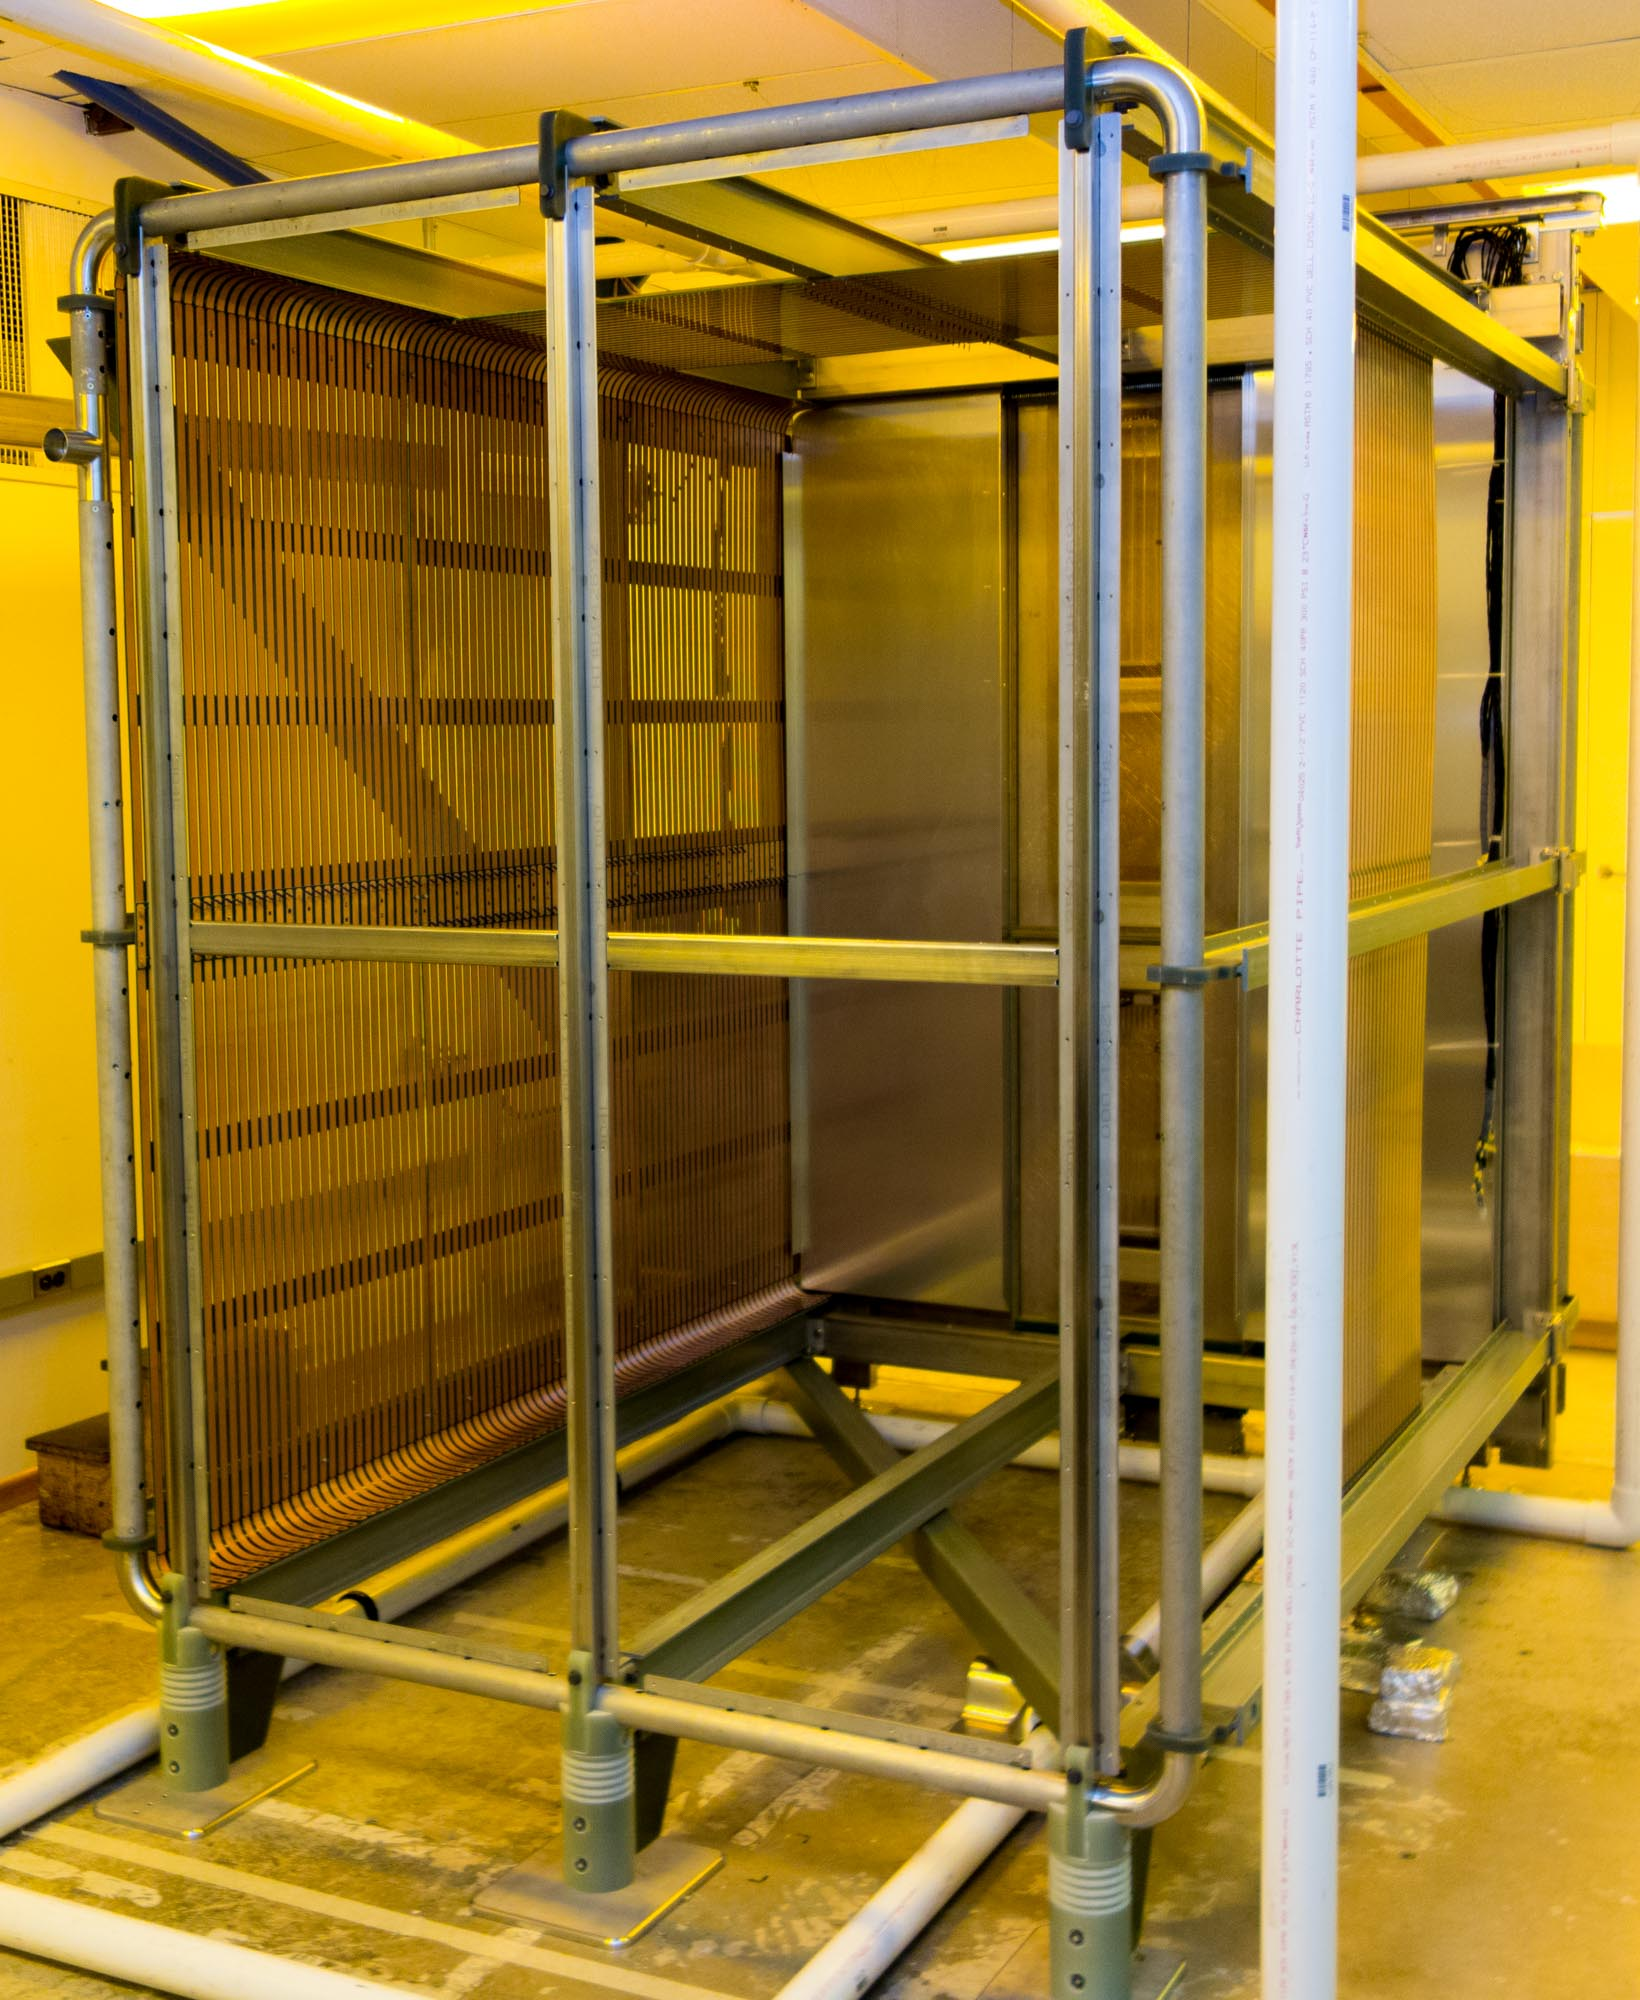
\includegraphics[width=0.35\textwidth]{35TTrial}
\end{cdrfigure}
\fixme{in fig 9.4 the APA is not labeled; I guess we all know it's the purple plane; if I'm wrong, it needs labeling!}

The Phase-2 prototype incorporates many of the design elements for the DUNE single-phase
far detector described in previous sections of this document.
In many cases, these include novel features that have never previously been tested in an operational TPC.
Some of the more important aspects are collected in Table~\ref{tab:35TDesign}.

\begin{cdrtable}[35-t Design Elements]{lcl}{35TDesign}{35-t Design Elements}
 Design Aspect& Section & How Tested\\ \toprowrule
Modular APAs with wrapped wires & \ref{subsec:fd-ref-apa}&Build small-scale APA Modules with FD design\\
\colhline
Vertical Gaps between APAs &\ref{sec:detectors-fd-ref-tpc}& Assemble APAs side-by-side.\\
&&Study reco'd tracks that cross the gaps.\\
\colhline
Horizontal Gaps between APAs &\ref{sec:detectors-fd-ref-tpc}& Build two shorter APAs and stack vertically\\
&&Study reco'd tracks that cross the gaps\\
\colhline
Field cage constructed of &\ref{sec:detectors-fd-ref-tpc}&Operate at HV
and measure field uniformity\\
FR4 Printed Circuit Board \\
\colhline
APAs immersed in active volume &\ref{sec:detectors-fd-ref-tpc}& Study reco'd tracks that cross APAs\\
\colhline
Cold Digital Electronics & \ref{sec:detectors-fd-ref-ce} & Measure noise performance etc. {\it in situ}\\
\colhline
Waveguide-style Photon Detector& \ref{sec:detectors-fd-ref-pd}&Install in APAs. Measure lightyield\\
\colhline
Triggerless-capable DAQ & \ref{sec:detectors-fd-ref-daq} & Take data using multiple DAQ modes\\
\end{cdrtable}

As can be seen from Table~\ref{tab:35TDesign}, successful tests of many of the new
design features will require simulation, reconstruction and analysis of 35-t data.
This will be performed using the LArSoft package, which is also used to simulate and
reconstruct data from ArgoNeuT, MicroBoone, and LArIAT.
Reuse of software developed for those experiments will greatly facilitate 35-t developments,
however, the novel hardware features of the 35-t prototype necessitate new software developments
as well; among them
\begin{itemize}
\item{code to divide the wrapped wires into as many as five individual linear segments.
A hit on a single electronic channel can, in principle, be related to a
signal on any of these segments.}
\item{``disambiguation'' code to identify which of the possible wire segments was actually responsible
for the observed hit}
\item{code for determining the start time of the event ($t_0$). Since the 35-t prototype DAQ can
run ``triggerless,'' methods are needed for finding the $t_0$ in data. Information from the external
scintillator paddles as well as the internal photon detectors can be used.}
\item{Code for ``stitching'' together track segments observed in different tracking volumes.
Since hits can come from either side of the four APAs, there are
effectively eight separate tracking volumes,
which are treated as separate TPCs.}
\end{itemize}

With these simulation and reconstruction tools in hand, ``physics'' analysis of the data can be undertaken
in the areas of %both 
validation of new detector design elements and analysis of basic LArTPC performance. % are needed.
Among the highest-priority analysis tasks are:

\begin{itemize}
\item{basic detector performance: signal/noise, purity measured with tracks, track direction resolution,
photon detector light yield}
\item{measurement of distortions due to space charge and field non-uniformity}
\item{identification of different types of particles: muons, protons, neutrons, pions}
\end{itemize}

The results obtained by operating and analyzing data from the 35-t Phase-2 prototype are expected
to be very valuable in refining the CERN single-phase prototype design, in preparation for the first \ktadj{10} DUNE far detector module.
